\documentclass{news}

\lang     {english}
\title    {The Ai Times:}
\subtitle {News, rumors, revelations, and prophecies from the age of artificial intelligence.}
\authors  {Alshival}
\keywords {newspaper, stories, journalism}
\date     {\today}
\location {Universal}
\cost     {}
\issue    {1}
\volume   {3}

\begin{document}

% \by{Samuel Cavazos}{Data Scientist}{../media/brain1_transparent_256x256.png}

\by{Samuel Cavazos}{Top 100 Data \& Analytics Professional}{../media/ait.png}

\hh{OpenAi's GPT-5.6 and Federal Oversight}
{\l{Y}ou are probably not on the list of people who will be able to access GPT-5.6, OpenAi's newest frontier model. Neither is \textit{The Ai Times}. \href{https://www.theverge.com/ai-artificial-intelligence/957372/openai-will-delay-gpt-5-6-after-trump-administration-request}{The Verge reports} that OpenAi is starting with a limited preview for a small group of enterprise customers after a Trump administration request, with the federal government approving customer access case by case.
\par} 

The line worth pinning down came from Sam Altman. \href{https://www.theguardian.com/technology/2026/jun/26/openai-ai-model-release-trump-us-sam-altman-gpt-anthropic-mythos}{The Guardian reported} that Altman told staff the government would be ``approving access customer by customer during this preview period.'' He also wrote that this was \href{https://www.axios.com/2026/06/25/trump-administration-openai-gpt-model-release}{``not our preferred long term model''} and that OpenAi would work with government and industry on a more sustainable release process. That is more precise than saying the government is controlling customers: the government is helping decide which customers get through the gate.

This is already becoming an industry pattern. \href{https://www.euronews.com/2026/06/27/anthropic-cleared-to-restore-mythos-5-access-to-certain-us-organisations}{Euronews reports} that Anthropic has been cleared to restore Mythos 5 access to certain U.S. organizations that operate and defend critical infrastructure, after an earlier directive forced Anthropic to shut off access to Fable 5 and Mythos 5 entirely. \href{https://www.reuters.com/world/us/us-presses-meta-agree-ai-reviews-security-concerns-rise-nyt-reports-2026-06-23/}{Reuters, citing the New York Times, reported} that the administration has also pressed Meta to agree to voluntary reviews that would let the government evaluate its models' abilities and vulnerabilities. There is a real safety argument for staging access to frontier models. But customer-by-customer approval is not just safety testing; it is distribution policy. Washington is no longer only asking whether a model is dangerous. It is helping decide who gets the best tools first.

\hh{Atoms for Thee, Branding for Me}
{\l{T}he man who spent years selling a product called ``Full Self-Driving'' has discovered that names should describe physical reality. \href{https://wccftech.com/elon-musk-calls-ibms-0-7-nanometer-chip-naming-misleading-says-atoms-should-decide-process-node-labels/}{Wccftech reports} that Elon Musk called IBM's 0.7-nanometer chip naming misleading, arguing that process nodes should be named by the number of atoms across the smallest feature. For once, the complaint is not wrong: IBM itself said 7 angstroms describes a generation of chips, not the old-school width of the contacted metal wires.
\par}

The funny part is the messenger. During \href{https://ir.tesla.com/webcast-2026-04-22}{Tesla's April 22 Q1 2026 earnings call}, Musk acknowledged that Hardware 3 vehicles cannot achieve unsupervised Full Self-Driving. \href{https://www.theverge.com/transportation/917167/elon-musk-tesla-hw3-fsd}{The Verge reported} that HW3 has only one-eighth the memory bandwidth of Hardware 4. Many people bought ``Full Self-Driving'' years before Tesla tacked on "supervised" to the name and thought the hardware could deliver the literal thing they paid for: full self-driving.

If atoms should decide chip labels, maybe cars with Hardware 3 should not carry the FSD label if ``Hardware 3 simply does not have the capability to achieve unsupervised FSD''.

\hh{The Pocket Dev Machine, Almost}
{\l{I} have always wanted a dev machine that fits in my pocket. A linux terminal, always accessible anywhere I go. That is powerful. The exact device to scratch that itch still does not exist, but we have all the pieces needed to simulate such a device. This past week, I had to wait 40 minutes at a movie theater, so I pulled out my foldable phone, a Samsung Galaxy Fold 7, connected to my home VPN, opened The Windows App, and RDP'd into my home supercomputer. 
\par}

\begin{center}
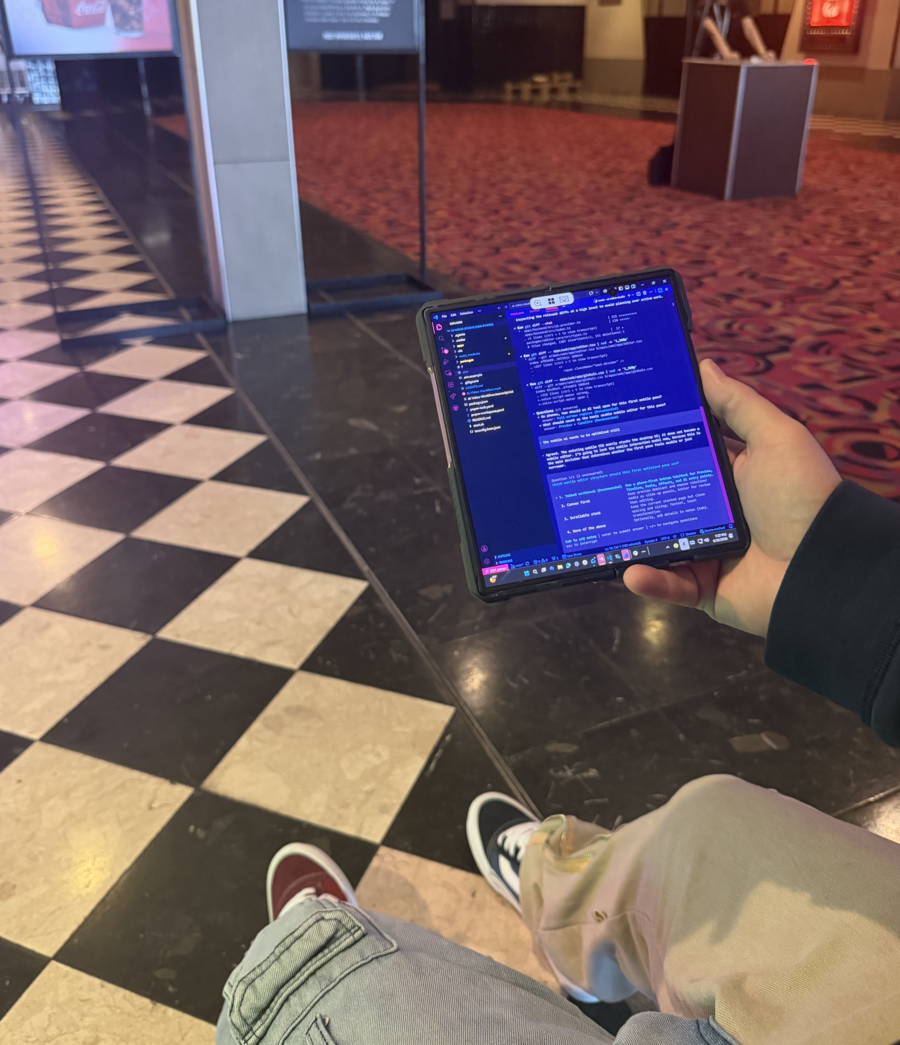
\includegraphics[width=\linewidth]{../media/pocket-dev-theater.png}
\end{center}

The size of the foldable screen was just the right size. I could hold it in my hand as I talk with friends and passively code. I felt comfortable, even. I had a terminal open and would send prompts, working on app architecture and chatting with friends as the agent worked through the changes. The phone becomes a window into a real machine with a GPU, all my files, all my tools, and enough horsepower to let an Ai prompt keep running after I close the app and walk into the theater. 

This is not local development on a phone, and I am not pretending it is. But for now, a foldable phone remote desktop plus VPN plus a home workstation gets me most of what I actually wanted: start a task anywhere, let the big machine chew on it, and pick it back up later at my desk. When I need something portable but powerful enough to run a local dev environment, my Asus Xbox ROG Ally X is the way to go. Handheld gaming devices serve as great portable dev machines, which is why I buy ROG/Legion handhelds for my interns. 

Getting the foldable phone to work requires an investment. Many ISP no longer assign residential accounts static IP addresses, requiring an expensive business plan. Then you need to set up the VPN (some asus routers make this easy with OpenVPN). And so much more. So it's great, but still not scratching that itch. A foldable phone with a linux subsystem would be ideal. One that runs VS Code locally.

\hh{Announcements}

\textit{The Ai Times} is now on Substack. Scan the code below to get each new issue, along with the sources, side quests, and stray prophecies that did not fit on the page.

\begin{minipage}[c]{.50\linewidth}
{\large\cinzel
{\normalsize The }

\qquad Ai

\qquad\quad Times}
\end{minipage}%
\begin{minipage}[c]{0.50\linewidth}

\includegraphics[width=\linewidth]{../media/ai-times-qr.png}
\end{minipage}

\end{document}
